\section{Computing Continuum}
\label{sec:example}

Herein we will discuss the challenges of developing an application that exploits the computing continuum. 

























%TODO Update the legenda: should be AV (Autonomous Vehicle) instead of CV 
\begin{figure}[tbp]
	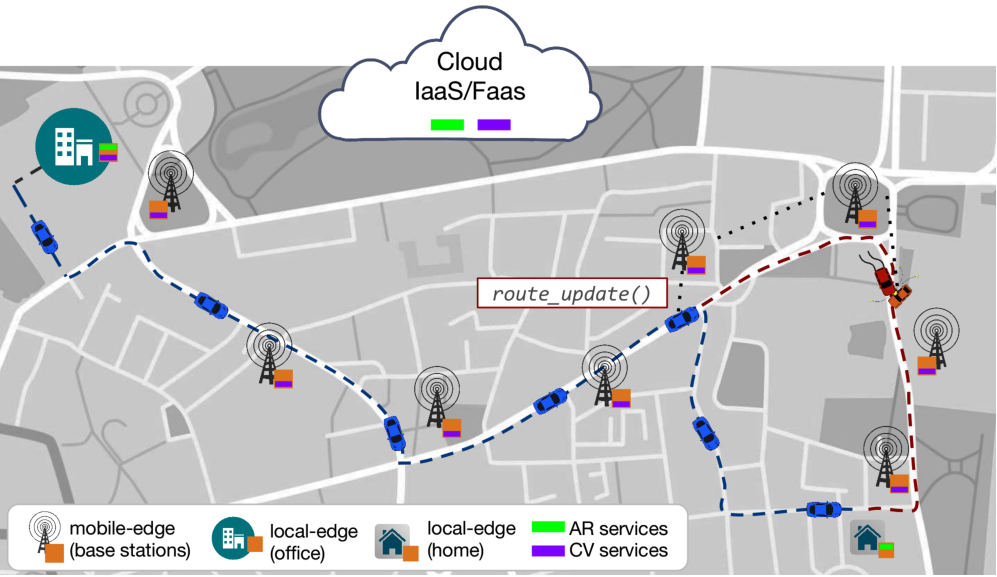
\includegraphics[width=0.9\textwidth]{figs/Continuum-Scenario}
	\caption{Heterogeneous applications such as Augmented Reality (AR) and Autonomous Vehicles (AV) interact with services deployed along the computational continuum (cloud, mobile-edge, local-edge, and mobile)}
	\label{fig:continuum-scenario}
\end{figure}

%Throughout this section an example scenario (Fig.~\ref{fig:continuum-scenario}) is used to illustrate the use of A3-E model and the cloud-edge-mobile continuum with different applications employed by a person with visual impairment.
We illustrate the computational continuum in an example scenario (Fig.~\ref{fig:continuum-scenario}) that starts in a user's office and finishes at her home. It involves different applications that rely on services executed in the cloud, edge, or in the user's own devices. 

First, let us assume the existence of a local edge server in the user's office (hereafter called \textit{local-edge}). This server is owned by the company, and it is used to extend the computational capabilities of the devices operated by its employees. In our example, the user makes use of an augmented reality (AR) application to craft virtual 3D objects that are added to her desk table. This application involves heavyweight image processing for 
the \textit{extraction of features} from the captured scenes, as well as a trained neural network model to \textit{detect objects} from a set of features. With the offloading of both tasks to the local-edge, the user can avoid recharging her glasses and can improve her productivity. Also, the additional storage on the edge servers allows a larger set of objects to be recognized, thanks to a more completely trained model.

After work, the user leaves her offices and enters her autonomous vehicle (AV). During her way home, the vehicle makes use of services deployed at edge servers located at cellular base stations (hereafter called \textit{mobile-edge}) to receive low-latency updates about the best plan to reach her destination. This way, within milliseconds the vehicle can be suggested to adjust its routes to avoid heavy traffic. In particular, let's say that a new path consists of residential streets without mobile-edge coverage. The AV continues to fetch updates, which are now served by a cloud provider. The additional network latency is compensated with the low speed limit of the residential area.

Finally, at home the user can start using her domestic local-edge server. She finds out about a new mobile game application. Upon installation, the local-edge server becomes aware of a new continuum-compliant application and, while the app continues to run locally on her device, it proceeds to setup the services needed to allow the application to offload some of the computation. Once the setup is complete, the application autonomously starts using the edge services with the purpose of preserving the device's resources. Not only does the game's performance improve, battery consumption is also reduced.  

This scenario exploits different parts of the continuum. Cloud services are employed as a reliable alternative to edge services. Similarly, local services are employed as alternatives to edge services until they have been acquired and made available by a local-edge server. Whilst the transition between mobile-edge and cloud was transparent, the use of local-edge services involved the mutual client-server awareness.